\section{Fast grasp planning for familiar objects}
\label{cha3:sec2}

Traditional manipulation planning strategy usually involves inverse kinematics and optimization, which are computationally expensive. The reported computation time varies from 0.1 seconds to a few minutes. Recently, there have been some attempts to tackle the problem with real time solutions. \citet{Richtsfeld2008} use a laser scanner to detect cylindrical shapes and plan grasps. This method is limited to cylindrical objects. Kanehiro et al.~\citep{harada2008fast} use approximation models of the friction cone and roughly estimate the force closure criterion. However, this approximation may limit their solutions. In the planning step, they use random sampling techniques to generate grasping postures and loop through the samples to find a grasp satisfying all the kinematic constraints. The reported computation time varies from 10$sec$ to 25$sec$ including path planning of the arm using a 2GHz core.
Daoud et al.~\citep{daoud2011fast} employ a genetic algorithm optimization approach to provide an initial grasp before online manipulation. This evolutionary approach relies on several iterations of optimization before reaching the solution. The reported time is 12.61$sec$ for a spherical object with a 2.2GHz core. The latter two methods, due to their iterative approaches, do not guarantee fast computation in all cases. In contrast, with our closed-form solution the computation time is bounded within a few milliseconds.

We avoid using these by adopting a learning approach.
Our method for planning grasps for familiar objects starts by generating a training dataset of stable grasps for the objects. A $Gaussian$ $Mixture$ $Model$ (GMM)~\citep{cohn1996active} is learned from the data, and the target pose is predicted via $Gaussian$ $Mixture$ $Regression$ (GMR). Hence there is no inverse kinematics computation nor iterative optimization in our method. Generally speaking, our approach is to:
\begin{enumerate}
\item Generate a set of stable grasping demonstrations for a given object and a robot hand (Section~\ref{cha3:sec2:demonstration}).
\item Build a statistical model for the training dataset offline (Section~\ref{cha3:sec2:learn}).
\item Use the model to quickly generate a new grasp, given a starting object-hand configuration (Section~\ref{cha3:sec2:plangrasp}).
\end{enumerate}

\subsection{Grasp generation given the hand kinematics}
\label{cha3:sec2:demonstration}

Two robot platforms available in our lab are chosen to perform the grasping tasks: the iCub and the Barrett hand. The iCub has an anthropomorphic hand with 9 degrees of freedom: 3 in the thumb, 2 in the index, 2 in the middle finger, 1 in the ring and little fingers and 1 for the adduction/abduction movement (Figure~\ref{fig:robothand}(a)). The Barrett hand is an industrial grasper with 3 fingers and 4 degrees of freedom: 1 for each finger and 1 for the separation between the second and the third finger (Figure.,~\ref{fig:robothand}(b)). These two platforms differ drastically in the range of motion for each finger and provide very different grasp demonstrations. They will hence grasp objects in very different ways.

\begin{figure}
  \centering
  \subfloat[\scriptsize{iCub hand}]
  {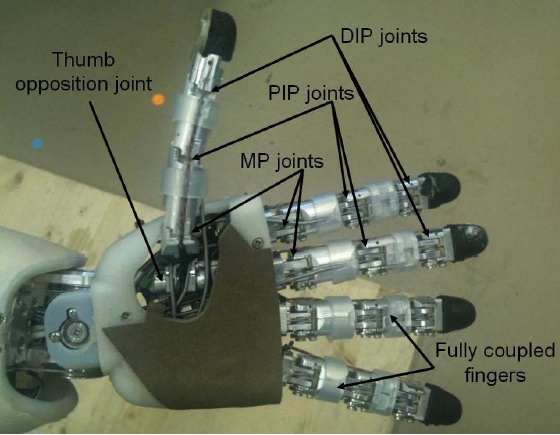
\includegraphics[height=4.5cm]{./fig_cha3/icubhand.jpg}}
  \subfloat[\scriptsize{Barrett hand}]
  {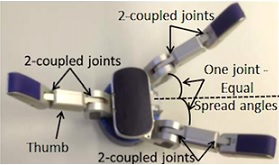
\includegraphics[height=4.5cm]{./fig_cha3/barretthand.jpg}}
  \caption{Two robot platforms used in this work. This method is not bounded to these two robots. It can be applied to any other robot hands given their kinematics.}
  \label{fig:robothand}
\end{figure}

Starting from the geometry of an object and the kinematic property of a robot hand to compute a feasible grasp is time consuming. To achieve fast planning, we do this computation offline. There are numerous possible ways to grasp one object depending on the task's needs~\citep{sahar2012,el2013generation}. To encapsulate all the possible ways, a large amount of training data is needed. Collecting this amount of data on a real robot is time consuming. Therefore, instead of using a real robot, we generate training data by synthesis.

Two different approaches are used here: optimization and simulation. We use simulation method for the Barrett hand and use optimization method for the iCub hand. In simulation, we use a trial-and-error approach: in the state space we try to generate as many grasps as possible and select those feasible ones. In principle we can generate more variety of grasps by this method, as some of them might be hard to reached by optimization. The 4 d.o.f Barrett hand is particularly suitable for this approach. For the 14 d.o.f iCub hand, however, the state space is much larger and hence the trial-and-error approach is expensive. Instead, for the iCub hand we use an optimization method.


%\subsubsection{Optimization}
\paragraph{Optimization}
~\\
We use the optimization algorithm proposed in the work of El-Khoury and etc.~\citep{el2013generation} to generate grasps for the iCub.
The iCub hand is modeled in 8 dimensions in this algorithm and the thumb, index and middle finger are taken into account.

This optimization algorithm formulates the problem as a constraint-based minimization for a set of hand configuration parameters (hand position \textbf{\emph{h}}, hand orientation {\textbf{\emph{o}}} and finger joints {\boldsymbol{$\theta$}}). These parameters are subjected to a number of constraints to satisfy the following criteria:

\begin{enumerate}
\item The grasp is kinematically feasible for the robot hand;
\item The grasp is a force-closure grasp;
\item The robot hand is not penetrating the object;
\item The robot fingertips contact the object surface;
\item The force provided by the robot hand is able to raise the object.
\end{enumerate}


The iCub's finger joints can only apply a limited amount of torque.
The less joint torque required, the easier it is for the iCub to lift the object. For this reason, we choose the objective function to be the minimum joint torque required to balance the gravity wrench, formulated as:
\begin{equation}
J(\boldsymbol{h},\boldsymbol{o},\boldsymbol{\theta})=\Arrowvert \sum_{i,j} {{\tau}^j_i}\Arrowvert
 \label{quality}
 \end{equation}
where {$\tau$}$^j_i$ is the $i$th joint torque of the $j$th fingers under the force feasibility constraints:

\begin{equation}
 {\tau}^j_i \in [\bar{\tau}^j_i, \hat{\tau}^j_i]
 \label{quality}
\end{equation}
where $\bar{\tau}^j_i$ and $\hat{\tau}^j_i$ are the lower and upper boundaries of $\tau^j_i$.
Minimizing this cost function is equivalent to minimizing the energy required in the joint space in order to accomplish the grasping task.
%As different grasps can cost similar amounts of energy, this objective function has many local optima and hence can provide a large set of different grasps.

The optimization is solved by the Interior Point OPTimizer (IPOPT) method proposed by W\"{a}chter and Biegler~\citep{wachter2006implementation}, written in the AMPL Model Language for Mathematical Programming. To generate a variety of grasps, we exploit the fact that the IPOPT solver converges to local solutions. We provide the solver with a large number of initial conditions, varying from 1000 to 2000. From these initial conditions, which are located in different areas of the space, the IPOPT converges to their corresponding local optima. By this means 500 to 1000 optimized grasps for an object can be obtained. They will be used as the training data in the next phase. The average computation time for the IPOPT to converge to one solution is 2.65$sec$, with a standard deviation of 1.82$sec$. As additional information, the quality $Q$ of each optimized grasp is calculated in the form described in~\citep{ponce1997computing}:

\begin{equation}
Q =\Arrowvert \frac{1}{3}\sum_{j} {\boldsymbol{c}^j}\Arrowvert
\vspace{-0.1in}
\end{equation}
where \textbf{\emph{c}}$^j$ is the contact point (i.e. fingertip) position of the $j$th finger. Though it is not included in the optimization, the quality is used in the comparison between the training set and the result set shown in Section~\ref{cha3:sec3}.

%, by the distance from the grasp polyhedron to the center of mass of the object:

%To measure the quality of the optimized grasps, the quality $Q$ is calculated as described in~\citep{ponce1997computing}, by the distance from the grasp polyhedron to the center of mass of the object:

To ensure the robot fingertips contact the object surface, the object has to be expressed by an implicit equation. For example, a cylinder can be expressed as:

\begin{equation}
{\left(x^2+y^2\right)}^{10}+z^{20} = 1
 \label{equ:cylinder}
\end{equation}

During optimization, this will be used as an hard constraint for the all the fingertip position.
For more complex shapes, the implicit equation can be learn by Gaussian process~\citep{el2013generation}.

The algorithm above can generate a variety of high quality force-closure grasps for a given robot hand kinematic structure and an object model. Since IPOPT is a continuous optimization solver, generating grasps on complex objects requires a continuous implicit representation of the whole object surface model.

%Representing complex objects as an assembly of superquadrics induces a discontinuity in this model preventing IPOPT from converging to a feasible solution.
%An implicit object representation for grasp generation using optimization will be addressed in our future work. This paper will only focus on grasps generated, for the iCub hand, on simple shaped objects such as a cylinder and cuboid.



%\subsubsection{Simulation}
\paragraph{Simulation}
~\\
%TODO: quality criterion: Ferrari and Canny
As the Barrett hand is modeled in the widely used simulator GraspIt!~\citep{miller2004graspit}, we use simulation to generate its data. GraspIt! is designed for grasp analysis and it provides a library of robots and object models. Its quality measurement module computes the grasp quality according to all the contacts between the hand and the object, in the form described by Ferrari and Canny~\citep{ferrari1992planning}. A grasp planning module for primitive shapes, i.e cylinder, sphere, cuboid and cone, is available, allowing users to easily generate grasps~\citep{miller2003automatic}.
To sample grasps for objects with complex shapes, we alter the module and generate grasps as follows.

\begin{figure}
  \centering
  \subfloat[\scriptsize{Initial distribution}]  {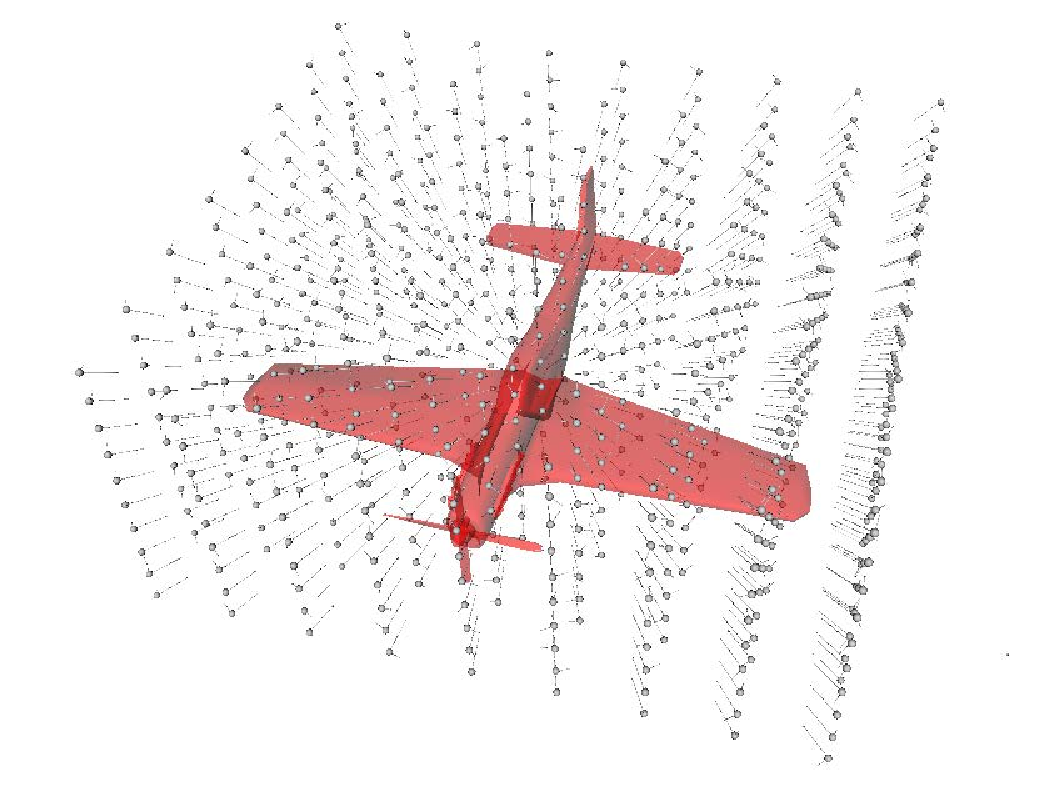
\includegraphics[width=7cm]{./fig_cha3/plane_x2_lattice1.pdf}}
  \subfloat[\scriptsize{Final distribution}]  {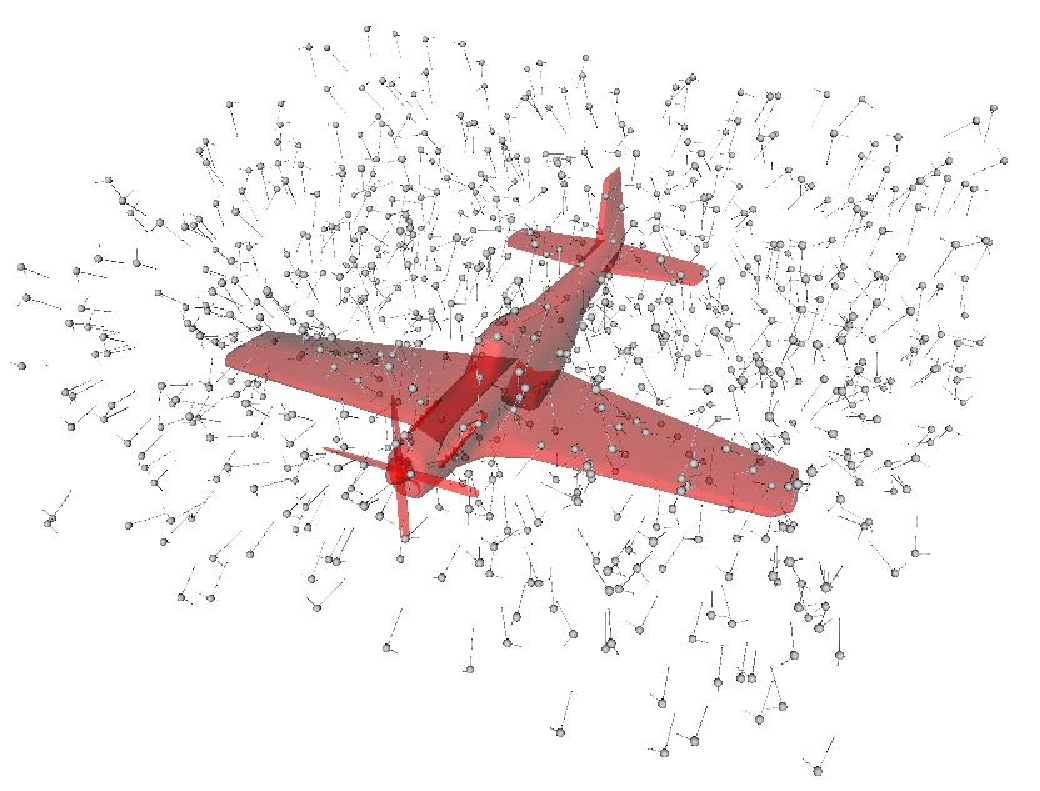
\includegraphics[width=7cm]{./fig_cha3/plane_x2_lattice2.pdf}}
  \caption{\scriptsize{An illustration of part of the grasp position lattice of an airplane model. Each grey dot in the lattice represents one robot hand position. The long arrows at each dot represent the hand normal directions and the short arrows represent the fix finger directions. The hand normals are initialized by pointing toward the center of the object, as shown in (a). Small random variance is then added to each grasp later to even the distribution and the final distribution is shown in (b).}
}
    \label{lattice}
\end{figure}

Firstly a robot hand position ``lattice" is generated. Each vertex in the lattice represents one robot hand position, where the hand will be placed to grasp the object (Figure~\ref{lattice}). The object is located in the center of the lattice surrounded by the grasping positions. All palm normals are initially pointing to the center of the object. Random finger separation angles are assigned to each point to form a list of grasp configurations for testing. According to the object size, 1000 to 20000\footnote{More complex and bigger shapes need more testing points.} testing grasps can be generated to ensure that the entire object is surrounded by the lattice and the farthest point to grasp the object is included. The density of the hand position lattice depends on the object shape. Objects with sharp edges, where the normals on the surface change sharply, should have a higher lattice density compared to those with smooth surfaces.

In the final step before testing, small random perturbations are added to each grasp so that the testing points are evenly and continuously distributed in all dimensions.
To test these grasps, the hand is first placed at each position on the test list with the desired posture (hand orientations and finger joints). Next, the fingers clutch around the object until contacts or joint limits prevent further motion. We then use the quality measurement module to compute the quality of each grasp. The non-zero quality grasps, i.e. force-closure grasps, are recorded and used as training data. Note that not all the testing grasps result in feasible grasps. Points causing collisions are removed from the list and only the force-closure grasps are kept as the training data. The average generating rate for the feasible grasps is roughly one per five seconds.

The Barrett hand has one joint in each finger. These three joints can only rotate in one direction and how much they rotate is determined by the object surface, given the hand position, orientation and the separation angle.
Therefore we drop this redundant information and model a Barrett hand grasp only with the hand position, hand orientation and the finger separation angle. The robot kinematics is programmed into the simulator and all simulated robot movement is feasible.

The above two methods can be used to generate both simple shapes and complex shapes. The size of the generated training data varies from 500 to 1600 (Table~\ref{result}). Each training dataset is split into 5 groups for the 5-fold cross validation in the later step.


\subsection{Model learning}
\label{cha3:sec2:learn}

The second phase of the approach is to build a model $\varOmega$ for the grasp demonstrations.
A $Gaussian$ $Mixture$ $Model$ (GMM) is used here to get a probabilistic encoding of the joint distribution $p$(\textbf{\emph{h}},\textbf{\emph{o}},\textbf{\emph{$\theta$}} \text{\textbar} $\varOmega$).
We choose to use GMM because of its ability to effectively extrapolate the missing data, as has been exploited in many applications~\citep{calinon2007learning,sauser2011iterative}. It also has the advantage of capturing the non-linearity of the space, as well as determining how likely a point in the input space is under the model.
The ability to estimate the likelihood of an input query point is crucial: an inference far away from the region covered by the training data can be unreliable, resulting potentially in an infeasible grasp. With GMM we are able to make sure that each input query point is located in or projected to a reliable region (this is explained in the next phase).

Therefore, in the grasp planing phase, we first make sure that a new query point locates in a reliable region by checking it likelihood.
Given a set of sample grasps represented by the hand position \textbf{\emph{h}},  orientation \textbf{\emph{o}} and the finger configuration \boldsymbol{$\theta$}, we model the distribution with a GMM as a sum of $K$ Gaussian components:

%$\xi$\{{\bf {\em h}},{\bf {\em o}},{\boldmath$\theta$}\}, we build our statistical model as a GMM:

\begin{equation}
{
P (\boldsymbol{h},\boldsymbol{o},\boldsymbol\theta \text{\textbar} \varOmega)
= \sum_{k=1}^K {p_{k}p(\boldsymbol{h},\boldsymbol{o},\boldsymbol{\theta} \text{\textbar} {\boldsymbol{\mu}_k}, {\boldsymbol{\Sigma}_k})}
}
\end{equation}
where $k$ is the number of Gaussian components, $p_k$ the prior of the Gaussian component and the $\boldsymbol{\mu}_k$, $\boldsymbol{\Sigma}_k$ the corresponding mean and covariance as:

\begin{equation}
{
\boldsymbol{\mu}_k = \begin{pmatrix}    \boldsymbol{\mu}_{h,k}     \\
                                        \boldsymbol{\mu}_{o,k}          \\
                                        \boldsymbol{\mu}_{\theta,k}
                    \end{pmatrix}
\hspace{0.2in}
\boldsymbol{\Sigma}_k = \begin{pmatrix}     \boldsymbol{\Sigma}_{hh,k}  & \boldsymbol{\Sigma}_{ho,k} & \boldsymbol{\Sigma}_{h\theta,k}  \\
                                            \boldsymbol{\Sigma}_{oh,k}  & \boldsymbol{\Sigma}_{oo,k}  & \boldsymbol{\Sigma}_{o\theta,k} \\
                                            \boldsymbol{\Sigma}_{\theta{h},k}   & \boldsymbol{\Sigma}_{\theta{o},k}   & \boldsymbol{\Sigma}_{\theta{\theta},k}
                        \end{pmatrix}
}
\end{equation}

A GMM approach requires that the data space is locally convex. For a complex object shape, however, the grasp space of hand configuration --- coupled with the finger joint space and constrained by the geometry of the object surface --- may be a non-smooth manifold. In both of the data generation methods described above, we evenly distribute the testing points so as to reduce the possibility of missing small good grasp regions. By these means we obtain most of the possible grasps for the object and approximate a locally convex data distribution, which is suitable for a GMM.

Before training we 1) convert all data into the object reference frame and 2) normalize the data so that all dimensions have a zero mean and a unit variance. Initialized by the K-means, the $Expectation$-$Maximization$ $algorithm$ (EM)~\citep{dempster1977maximum} is used to find the value of $\boldsymbol\mu$ and $\boldsymbol\Sigma$ that maximizes the probability of the training data under the GMM. The number of Gaussian $K$ is selected by the $Bayesian$ $Information$ $Criterion$ (BIC) and verified by 5-fold cross validation to make sure the model is not overfitting (Figure~\ref{bicxv}).

\begin{figure}
  \centering
    \subfloat[\scriptsize{BIC}]  {\label{fig:reachableSamplesPos}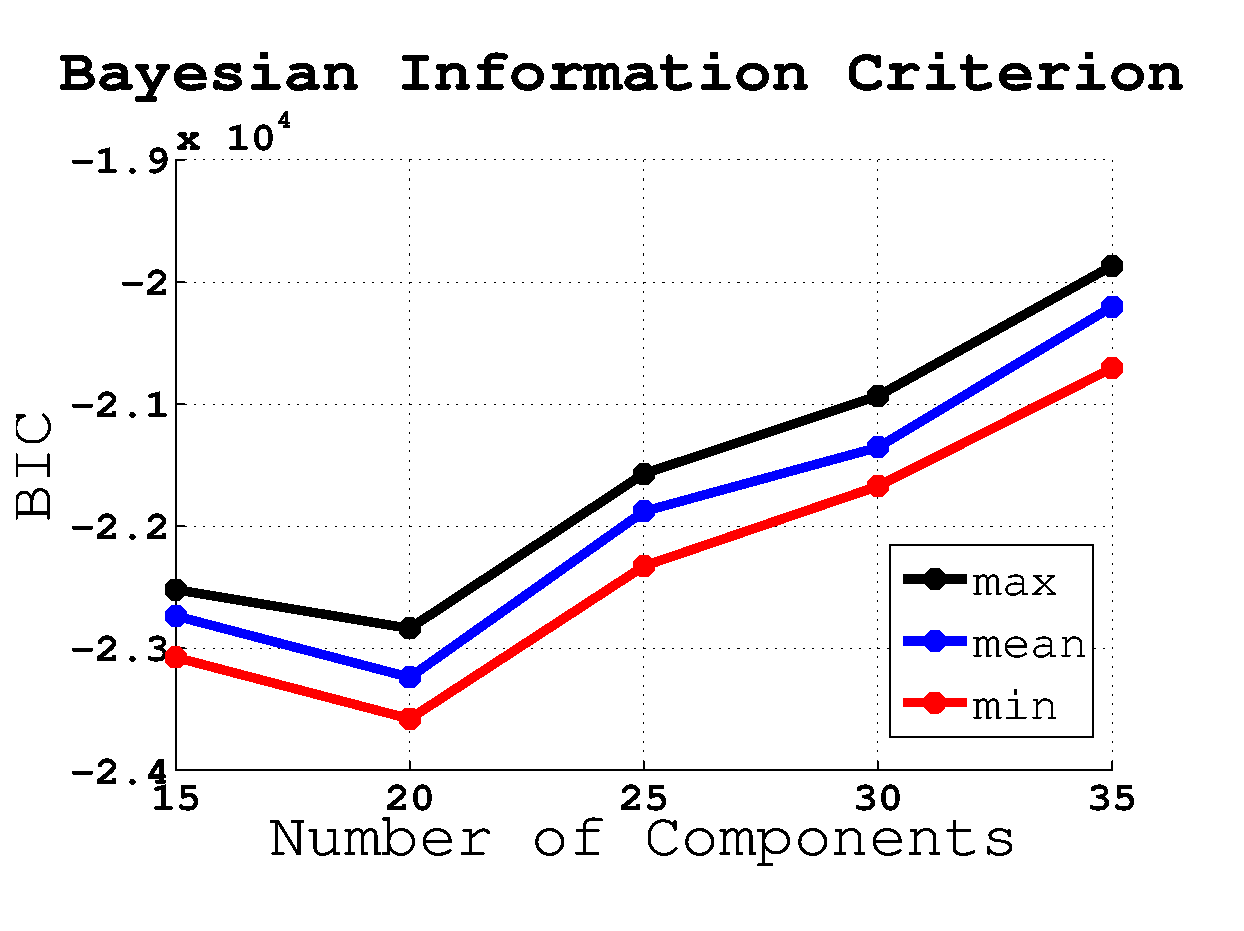
\includegraphics[width=7cm]{./fig_cha3/BIC.eps}}
    \subfloat[\scriptsize{5-fold cross validation}] {\label{fig:reachableModelPos}  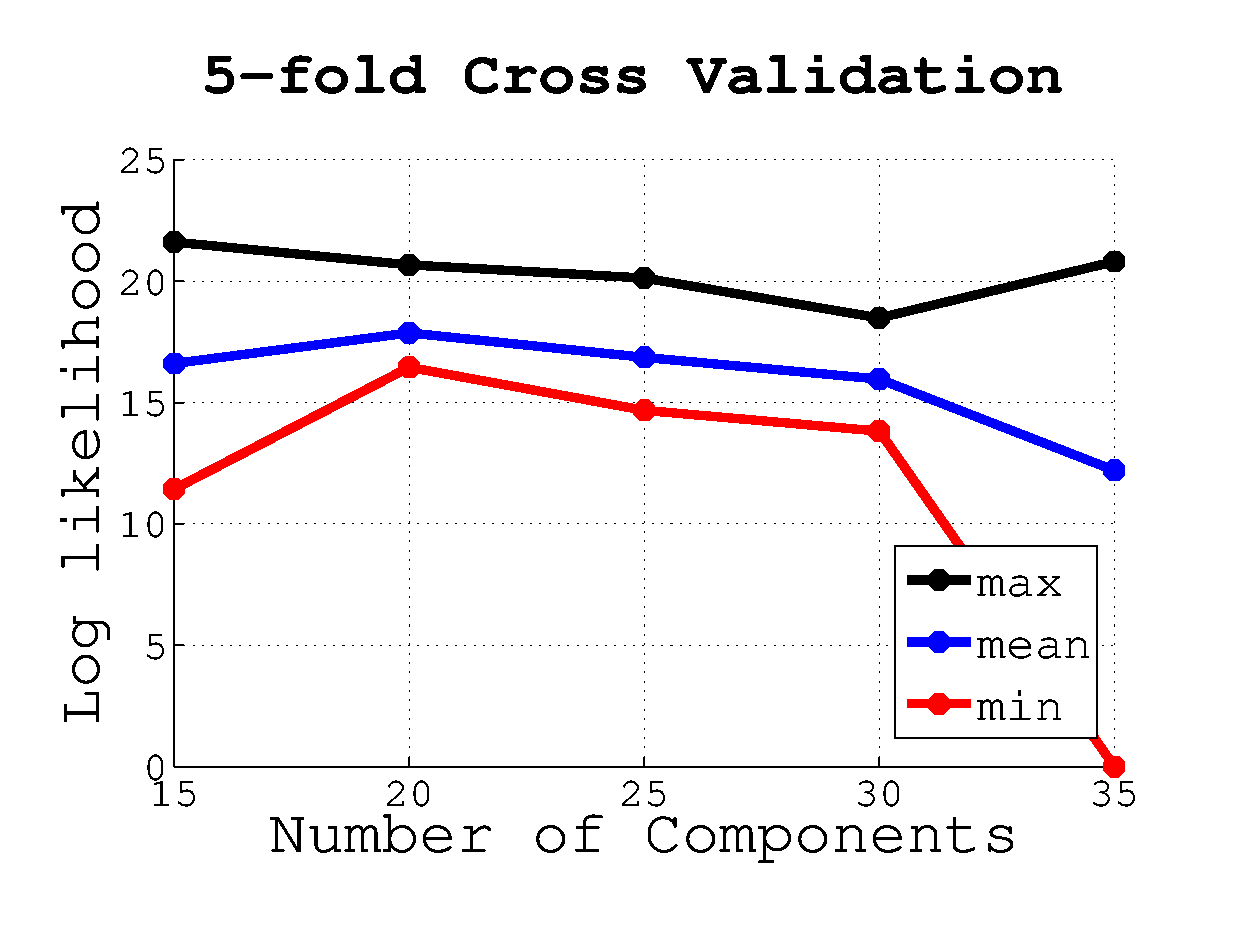
\includegraphics[width=7cm]{./fig_cha3/xValidation.eps}}

  \caption{\scriptsize{The $Bayesian$ $Information$ $Criterion$ and 5-fold cross validation test results of the training dataset of the Barrett hand and a joystick shaped object. For each number of Gaussians, the test is run 5 times. After empirical testing, the number of Gaussians is chosen to be 20. The corresponding experiment are shown in Section~\ref{cha3:sec3}.}
}
    \label{bicxv}
\end{figure}

\subsection{Grasp Planning}
\label{cha3:sec2:plangrasp}

With the learned GMM model of the grasping demonstrations, we plan a feasible grasp given a current hand configuration \textbf{\emph{q}}=\{\textbf{\emph{h}},\textbf{\emph{o}}\}. As discussed above, we first need to determine whether the \textbf{\emph{q}} is a valid query point. To do this we define a membership function $f$(\textbf{\emph{q}}) as:

\begin{equation}
f(\boldsymbol{q}) = \sum_{k=1}^{K}\bar{\boldsymbol{N}}(\boldsymbol{q};\boldsymbol{\mu}_k,\boldsymbol{\Sigma}_k)
\end{equation}
where $\bar{\boldsymbol{N}}$ is the normal distribution with the output being normalized between 0 and 1:

\begin{equation}
\bar{\boldsymbol{N}}(\boldsymbol{q};\boldsymbol{\mu}_k,\boldsymbol{\Sigma}_k) = exp\left(-\frac{1}{2}(\boldsymbol{q}-\boldsymbol{\mu}_k)^{T}\boldsymbol{\Sigma}_k^{-1}(\boldsymbol{q}-\boldsymbol{\mu}_k)\right)
\end{equation}

We consider a point to belong to the model if its Mahalanobis distance to any Gaussian component is less than a given threshold $\sigma$. In our experiments, we find that within 1~standard deviation the success rate of finding a feasible grasp is constantly high. For example in the Barrett hand and the model plane grasping task, the rate of producing a feasible and stable grasp within 1 standard deviation is 85\% (Table~\ref{result}) while it is 64\% within 3 standard deviations. On the other hand, it is possible that GMM encapsulates two different clusters of data within a single Gaussian, leaving the mean of the Gaussian at an infeasible point. This means getting closer to the means does not ensure a higher success rate. Taking this trade-off into account, we choose 1 standard deviation as our threshold, which gives us a cutoff criterion $\eta$ = $exp(-\frac{1}{2}\sigma^2)$. If the membership function of a point has a higher value than $\eta$, we consider this point as a valid query point. Note that the finger configuration $\boldsymbol\theta$ is not part of this input query point as $\boldsymbol\theta$ will be inferred by GMR later.

This membership function differs from the marginal likelihood $p$(\textbf{\emph{h}},\textbf{\emph{o}}) in two aspects. Firstly, it gives each Gaussian component the same weight, regardless of their priors $p_k$. As the prior of each Gaussian is proportional to the number of data points that are explained by this Gaussian, using this information in our selection may bias our choice toward the ``most popular" grasps, yielding less variety in the results.
Secondly, $\bar{\boldsymbol{N}}$ is a normalized function bounded between 0 and 1. This ensures the points with the same Mahalanobis distance from a Gaussian will have the same membership value, regardless of the size of the covariance~\citep{sauser2011iterative}.


In the case that \textbf{\emph{q}} is not a valid query point, we need to project it to a new point $\boldsymbol{q}^*$ that has a membership function value higher than $\eta$. Here we use a closed-form solution by considering each individual Gaussian component. We first compare the Mahalanobis distances between the query point \textbf{\emph{q}} and each Gaussian to find the nearest Gaussian component. The projection point $\boldsymbol{q}^*$ is found by projecting $\boldsymbol{q}$ to this nearest component (Figure~\ref{contour}).
%Point \textbf{\emph{q}} is then projected to this component to find the nearest point $\boldsymbol{q}^*$, which is less than one standard deviation away from the center of the Gaussian (Figure~\ref{contour}).
In the Mahalanobis space the Gaussian is in a uniform shape. As a result, the projection point $\boldsymbol{q}^*$  lays on the direction from the \textbf{\emph{q}} to the center of the Gaussian. Therefore the projection point $\boldsymbol{q}^*_k$ of the $k^{th}$ Gaussian can be written as:


\begin{equation}
\boldsymbol{q}^*_k = \boldsymbol{q} + \alpha_k(\boldsymbol{q}-\boldsymbol{\mu}_k)
\end{equation}
where $\alpha_k$ is a scalar. With $\sigma = 1$ and the equation

\begin{equation}
\bar{\boldsymbol{N}}_k(\boldsymbol{q};\boldsymbol{\mu}_k,\boldsymbol{\Sigma}_k) = exp(-\frac{1}{2}\sigma^2)
\end{equation}
we have the equation to easily compute $\boldsymbol{q}^*_k$:

\begin{equation}
-\frac{1}{2}(\boldsymbol{q}^*_k-\boldsymbol{\mu}_k)^{T}\boldsymbol{\Sigma}^{-1}_{k}(\boldsymbol{q}^*_k-\boldsymbol{\mu}_k) = -\frac{1}{2}\cdot{1}^{2}
\end{equation}

Once the projection point $\boldsymbol{q}^*$ is found, the $Gaussian$ $Mixture$ $Regression$ (GMR) is used to predict a feasible finger configuration $\boldsymbol\theta^*$ for it. First we define:

\begin{equation}
{
\boldsymbol{\mu}_{q,k} = \begin{pmatrix} \boldsymbol{\mu}_{h,k}    \\
                                        \boldsymbol{\mu}_{o,k}
                        \end{pmatrix}
\hspace{0.3in}
\boldsymbol{\Sigma}_{qq,k} =  \begin{pmatrix}  \boldsymbol{\Sigma}_{hh,k}  & \boldsymbol{\Sigma}_{ho,k}  \\
                                            \boldsymbol{\Sigma}_{oh,k}  & \boldsymbol{\Sigma}_{oo,k}
                            \end{pmatrix}
}
\end{equation}
and GMR then uses:

\begin{equation}
{
\hat{\boldsymbol{\mu}}_{\theta,k} = \boldsymbol{\mu}_{\theta,k} + \boldsymbol{\Sigma}_{\theta{q},k}(\boldsymbol{\Sigma}_{qq,k})^{-1}(\boldsymbol{q}-\boldsymbol{\mu}_{q,k})
}
\end{equation}

\begin{equation}
{
\hat{\boldsymbol{\Sigma}}_{\theta\theta,k} = \boldsymbol{\Sigma}_{\theta\theta,k} - \boldsymbol{\Sigma}_{\theta{q},k}(\boldsymbol{\Sigma}_{qq,k})^{-1}\boldsymbol{\Sigma}_{{q}\theta,k}
}
\end{equation}


Finally, all the $K$ components are taken into account and the target finger configuration $\boldsymbol{\theta}^*$ is predicted as the mean $\hat{\boldsymbol{\mu}}_\theta$ with the covariance $\hat{\boldsymbol{\Sigma}}_{\theta\theta}$ according to:

\begin{equation}
{
\hat{\boldsymbol{\mu}}_{\theta} = \sum_{k=1}^K{\beta_k(\boldsymbol{q}^*)}\hat{\boldsymbol{\mu}}_{\theta,k}
}
\end{equation}
\begin{equation}
{
\hat{\boldsymbol{\Sigma}}_{\theta\theta} = \sum_{k=1}^K{\beta_k(\boldsymbol{q}^*)}^2\hat{\boldsymbol{\Sigma}}_{\theta\theta,k}
}
\end{equation}
where
\begin{equation}
{
\beta_k(\boldsymbol{q}^*) = \frac{p_{k}p(\boldsymbol{q}^*|\boldsymbol{\mu}_{q,k},\boldsymbol{\Sigma}_{qq,k})}{\sum_{k=1}^K{p_k}p(\boldsymbol{q}^*|\boldsymbol{\mu}_{q,k},\boldsymbol{\Sigma}_{qq,k})}
}
\end{equation}

Due to the probabilistic nature of the GMR, the inferred result $\boldsymbol{\theta}^*$ is not a unique value but a mean value with variance. Though this mean does not guarantee a feasible solution, it provides a good estimation of a feasible one.

To find the closest Gaussian component we used the Mahalanobis distance rather than the Euclidean distance. The advantage of this is that it takes into account the correlations among each dimension of the hand configuration. In a space of different types of measurements, i.e. length and angle, Mahalanobis space is a better representation than the Euclidean space. Indeed, humans do not always use the Euclidean distance to select their grasps. We may move our hand further than needed to grasp an object, in order to avoid flipping our hand to another orientation. The performance of this method is discussed in the next section.

